\documentclass[]{beamer}
\usetheme{UniversiteitGent}

\usepackage{minted}
\usepackage{pgfplots}

\pgfplotsset{width = 7cm, compat = 1.8}
\usetikzlibrary{decorations.markings, snakes, trees}

\def\Point{36.9}

\begin{document}
\begin{frame}
  \frametitle{Inleiding}
\end{frame}

\begin{frame}
  \frametitle{Wat gaan we vandaag leren?}
\end{frame}

\section{Voorbeelden}

\begin{frame}
  \frametitle{\url{http://TeXample.net}}

  \begin{columns}
    \begin{column}{.4\textwidth}
      \begin{enumerate}
        \item 350+ voorbeelden
        \item gesorteerd in categorie\"en
        \item bestaat al 8 jaar
        \item heeft ook een lijst van interessante \LaTeX\ blogs
      \end{enumerate}
    \end{column}

    \begin{column}{.6\textwidth}
      \begin{flushright}
        \input{tikz/title-graphics.tikz}
      \end{flushright}
    \end{column}
  \end{columns}
\end{frame}

\begin{frame}
  \frametitle{\url{http://PGFPlots.net}}

  \begin{columns}
    \begin{column}{.4\textwidth}
      \begin{enumerate}
        \item 50+ voorbeelden
        \item gesorteerd in categorie\"en
        \item bestaat nu een maand
      \end{enumerate}
    \end{column}

    \begin{column}{.6\textwidth}
      \begin{flushright}
        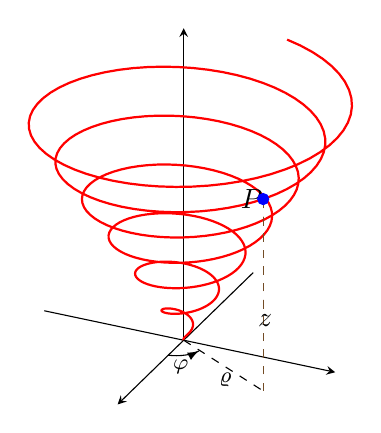
\begin{tikzpicture}
  \begin{axis}[
    view       = {-25}{-25},
    axis lines = middle,
    zmax       = 60,
    height     = 8cm,
    xtick      = \empty,
    ytick      = \empty,
    ztick      = \empty
  ]
  \addplot3+ [
    ytick      = \empty,
    yticklabel = \empty,
    domain     = 0:14.7*pi,
    samples    = 400,
    samples y  = 0,
    mark       = none,
    thick,
    red,
  ]
  ( {x*sin(0.28*pi*deg(x))},{x*cos(0.28*pi*deg(x)},{x});
  \addplot3+ [
    mark options = {color=blue},
    mark         = *
  ] 
  coordinates {({\Point*sin(0.28*pi*deg(\Point))},
    {\Point*cos(0.28*pi*deg(\Point)}, {\Point})};
  \addplot3+ [
    domain    = 0:12*pi,
    samples   = 100,
    samples y = 0,
    mark      = none,
    dashed,
  ]  
  ( {\Point*sin(0.28*pi*deg(\Point))}, {\Point*cos(0.28*pi*deg(\Point)}, {x} );
  \addplot3[
    mark=none,
    dashed
  ]
  coordinates {(0,0,0) ({\Point*sin(0.28*pi*deg(\Point))},
    {\Point*cos(0.28*pi*deg(\Point)}, {0})};
  \draw[
    radius = 80,
    decoration = {
      markings,
      mark= at position 0.99 with {\arrow{latex}}
    },
    postaction=decorate
  ] 
  (axis cs:0,10,0) arc[start angle=80,end angle=14] (axis cs:14,0,0);
  \node at (axis cs:20,0,30) {$P$};
  \node at (axis cs:24,0,7) {$z$};
  \node [font=\footnotesize] at (axis cs:20,17,0) {$\varrho$};
  \node [font=\footnotesize] at (axis cs:6,15,0) {$\varphi$};
  \end{axis}
\end{tikzpicture}

      \end{flushright}
    \end{column}
  \end{columns}
\end{frame}

\section{PGF/TikZ}

\begin{frame}
  \frametitle{Een uitgewerkt voorbeeld: een gelijkzijdige driehoek}

  In de \emph{Elementen van Euclides} (3e eeuw voor Christus) worden vele constructies in vlakke meetkunde beschreven. We gaan nu een voorbeeld uit de Ti\textit{k}Z manual bespreken:
  \begin{quote}
    Hoe construeren we een gelijkzijdige driehoek op een gegeven lijnstuk?
  \end{quote}
  %\input{tikz/triangle/result.tikz}
\end{frame}

\begin{frame}
  \frametitle{Euclides: de configuratie}

  \begin{columns}
    \begin{column}{.6\textwidth}
      \inputminted[fontsize = \scriptsize]{latex}{tikz/triangle/configuration.tikz}
    \end{column}
    \begin{column}{.4\textwidth}
      \emph{geen output}
    \end{column}
  \end{columns}

  \TikZ bevat vele libraries die bepaalde zaken gemakkelijker maken. In dit voorbeeld zullen we er vier gebruiken.
\end{frame}

\begin{frame}
  \frametitle{Euclides: de rechte $AB$}

  \begin{columns}
    \begin{column}{.6\textwidth}
      \inputminted[fontsize = \scriptsize]{latex}{tikz/triangle/1a.tikz}
    \end{column}
    \begin{column}{.4\textwidth}
      \begin{tikzpicture}
  \coordinate (A) at (0,0);
  \coordinate (B) at (1.25,0.25);
  \draw[blue] (A) -- (B);
\end{tikzpicture}

    \end{column}
  \end{columns}


\end{frame}

\end{document}
